%!TEX root = volumeFinal.tex 
\chapter{\label{chap:busca}Busca}

O área de busca dentro da IA visa a solução de problemas através de um conjunto de ações que alcancem o objetivo desejado. As técnicas de busca aceitam mais de uma soluções para o mesmo objetivo com conjuntos de ações diferentes \cite{intelligence2003modern}. 

Para avaliar o desempenho de uma técnica de busca exitem quatro medidas que devem ser analisados \cite{intelligence2003modern}:
\begin{itemize}
	\item Completude - Sempre que há uma solução, a técnica garante que será encontrada;
	\item Otimalidade - Esta técnica garante sempre encontrar a melhor solução para o problema;
	\item Complexidade de tempo - Qual o tempo para encontrar a solução;
	\item Complexidade de espaço - Quanto de memória é necessário para achar a solução.
\end{itemize}   

Com essas medidas é possível analisar as técnicas de busca para identificar quando é melhor utilizar uma técnica com determinadas características. 
\section{Busca adversaria}

A busca adversaria é utilizada para ambientes competitivos, como nos jogos. Como em um jogo o jogador, preferencialmente, não informa suas jogadas previamente, o ambiente se torna imprevisível, e com isso os objetivos dos jogadores entram em conflito, ambos estão em busca da vitoria. Como solução para esse problema é preciso gerar uma solução de contingencia para tentar antecipar as jogadas do adversário \cite{intelligence2003modern}. 

Para explicar como resolver esse problema, primeiro é preciso considerar um jogo com dois jogadores, um é chamado de MAX e o outro de MIN. O jogador MAX começa o jogo e o jogo e então é alternado uma jogada de MIN e uma de MAX até o final do jogo. Ao final do jogo, quem vence obtém uma recompensa positiva e quem perde uma negativa. Um jogo pode ser formalizado como \cite{intelligence2003modern}:

\begin{itemize}
	\item $S_{0}$ - O estado inicial, que especifica como o jogo se configura no inicio.
	\item Jogadores(s) -  Define qual jogador tem o movimento no estado.
	\item Ações(s) - Conjunto das ações possíveis em um estado.
	\item Resultado(s, a) - Um modelo de transição, que define o resultado da ação a aplicada ao estado s.
	\item Terminal(s) - Verifica se o estado é um estado onde o jogo terminou.
	\item Utilidade(s,p) - Define qual é o valor numérico para o jogo quando atingir um estado s terminal por um jogador p. 
\end{itemize}

O estado inicial, as ações e os resultados definem a arvore das jogadas para o jogo. A arvore representa em cada nodo um estado do jogo e cada ligação com os níveis de baixo são os estados resultantes após a execução de cada ação possíveis para o estado. A alternância entre as jogadas de MAX e MIN até chegar as folhas da arvore que correspondem aos estados terminais. Como o ponto de vista é do MAX, o valor de cada nodo folha representa o valor de utilidade para o MAX, e os maiores valores representam bons resultados para o MAX e ruins para o MIN. Com isso o caminho resultante indica que aquela ação será a melhor ação para o estado atual. Um exemplo de uma arvore pode ser visto na Figura \ref{fig:gametree}, considerando os valores contidos nos nodos folhas o valor de utilidade do estado, a figura mostra que a técnica escolhe o melhor valor, neste caso o mais alto, para o jogador. 

%\msr[inline]{colocar uma figura de uma game tree?}
\begin{figure}[ht]
	\centering
	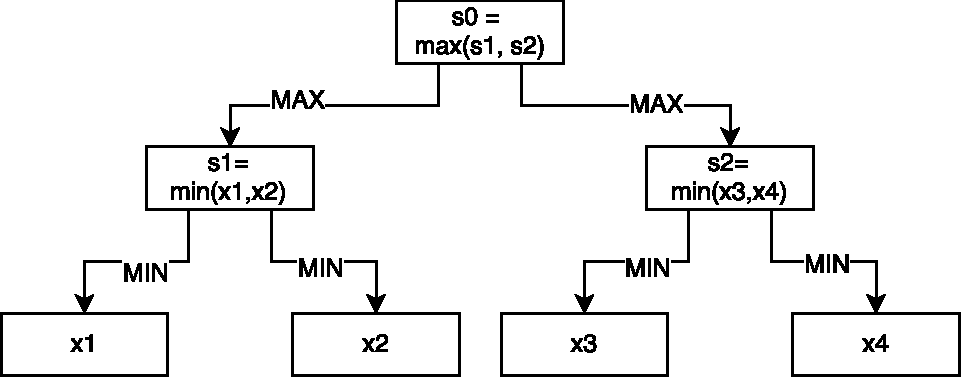
\includegraphics[width=0.6\textwidth]{fig/gametree.pdf}
	\caption{Exemplo de GameTree}
	\label{fig:gametree}
\end{figure} 

Este tipo de busca leva em consideração que o jogador adversário sempre realizará a jogada que mais lhe beneficiará. Um algoritmo que utiliza deste recurso é o algoritmo \textit{minimax search}, este algoritmo é completo por sempre achar uma solução e ótimo por sempre encontrar a melhor solução.
